% 
% Annual Cognitive Science Conference
% Sample LaTeX Paper -- Proceedings Format
% 

% Original : Ashwin Ram (ashwin@cc.gatech.edu)       04/01/1994
% Modified : Johanna Moore (jmoore@cs.pitt.edu)      03/17/1995
% Modified : David Noelle (noelle@ucsd.edu)          03/15/1996
% Modified : Pat Langley (langley@cs.stanford.edu)   01/26/1997
% Latex2e corrections by Ramin Charles Nakisa        01/28/1997 
% Modified : Tina Eliassi-Rad (eliassi@cs.wisc.edu)  01/31/1998
% Modified : Trisha Yannuzzi (trisha@ircs.upenn.edu) 12/28/1999 (in process)
% Modified : Mary Ellen Foster (M.E.Foster@ed.ac.uk) 12/11/2000
% Modified : Ken Forbus                              01/23/2004
% Modified : Eli M. Silk (esilk@pitt.edu)            05/24/2005
% Modified : Niels Taatgen (taatgen@cmu.edu)         10/24/2006
% Modified : David Noelle (dnoelle@ucmerced.edu)     11/19/2014

%% Change "letterpaper" in the following line to "a4paper" if you must.

\documentclass[10pt,letterpaper]{article}
\usepackage{authblk}
\usepackage{cogsci}
\usepackage{pslatex}
\usepackage{apacite}
\usepackage{physics}
\usepackage{graphicx}
\usepackage{amssymb}
\usepackage{amsmath}
\usepackage{caption}
\usepackage{subcaption}
\usepackage{booktabs}

\title{Evaluating machine comprehension of sketch meaning at different levels of abstraction}
 
%%% comment out authorship stuff for now

% \author[1]{\bf Kushin Mukherjee}
% \author[2]{\bf Holly Huey}
% \author[2]{\bf Xuanchen Lu}
% \author[3]{\bf Yael Vinker}
% \author[2]{\bf Rio Aguina-Kang}
% \author[2]{\bf Judith E. Fan}

% \affil[1]{University of Wisconsin-Madison, Madison, WI, United States}
% \affil[2]{University of California, San Diego, CA, United States}
% \affil[3]{Tel-Aviv University, Tel-Aviv, Israel}
\author{\bf Anonymous CogSci Submission}
\begin{document}
\makeatletter
\let\@oldmaketitle\@maketitle% Store \@maketitle
\renewcommand{\@maketitle}{\@oldmaketitle% 

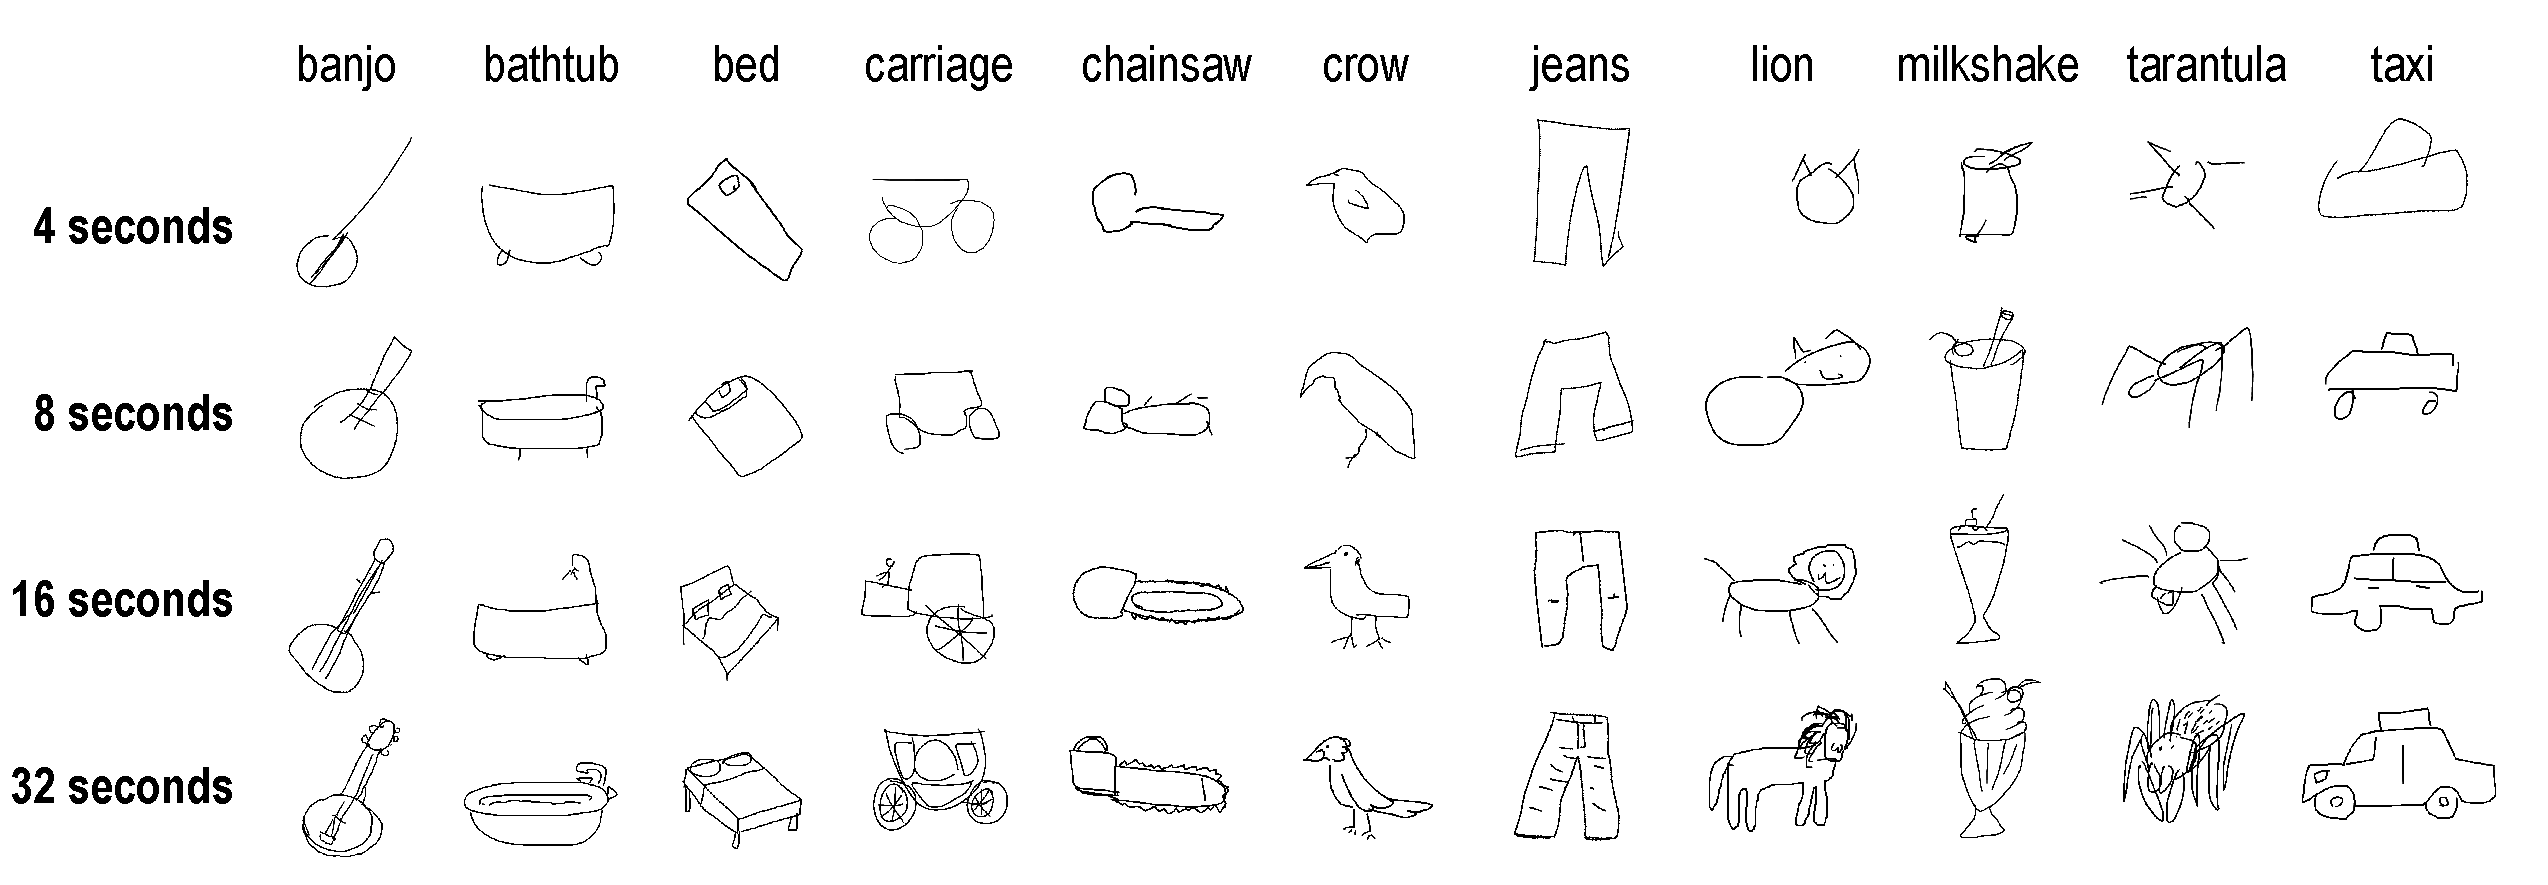
\includegraphics[width=.92\linewidth]{figures/thingsdraw_gallery_alpha.pdf}
\captionsetup{width=0.92\textwidth}
 \captionof{figure}{\footnotesize{Example sketches of objects from the THINGS128 dataset produced under different time limits.}}\

}
\makeatother
\maketitle

\begin{abstract}

People can understand sketches that vary in visual abstraction --- from detailed illustrations to schematic icons. 
To what degree are current vision algorithms sensitive to such variation when encoding their meaning? 
We first obtained $>80K$ human-generated sketches ($N$=5,563 participants) produced under different time limits (4s, 8s, 16s, 32s) and AI-generated sketches \cite{vinker2022clipasso} produced under different ink limits (8, 16, 32 strokes)  of 2048 real-world objects spanning 128 categories from the THINGS database \cite{hebart2019things}.
We then evaluated how 13 state-of-the-art vision algorithms varying in architecture and training represented the meaning of these sketches both at the category and exemplar levels without additional training.
We found that these models were generally sensitive to variation in visual abstraction, although some models were substantially more sensitive than others.
Together, these findings suggest promising avenues for building better models of human visual abstraction. 

\textbf{Keywords:} 
concepts; drawing; perception; computer vision; benchmark
\end{abstract}


\section{Introduction}
Humans have the ability to visually communicate their knowledge of the world—objects, scenes, and events—at varying levels of abstraction. 
Famously, the Spanish artist Picasso could both depict scenes with incredible detail and attention towards preserving the likeness to the real world, as well as depict concepts like ``dog'' with only a single stroke by omitting much of the information that would help the sketch share a visual resemblance to a real dog. 
Despite the striking differences in the level of detail and fidelity to the real world, both kinds of depictions can be understood and recognized by those who view them. 
This notion that knowledge can be flexibly expressed and comprehended at many such levels of abstraction, while raised in prior work  \cite{viola2017pondering, chen2020foundations,mccloud1998understanding}, has evaded a generalized formal account. 
As a consequence, it has remained unclear to what degree modern vision algorithms can support varied representations of the same underlying concept spanning multiple degrees of abstraction.

% While many might agree that knowledge can be flexibly expressed and comprehended at such different levels of abstraction, a formal account of visual abstraction has remained largely absent in the .


% For example, in the domain of sketching, a sketcher can choose to produce a highly-detailed realistic drawing or a simplified stylized drawing. 
% From an observer's perspective, the former might be evocative of a specific flower, such as a rose, the latter might convey the general concept of 'flower'. 

The relevance and necessity to abstract visually across many different levels arises across many instances of visual communication.
In certain contexts, a faithful and detailed depiction might be what is required, such as when an architect conveys detailed schematics to an engineer \cite{suwa1997architects} or when a zoologist creates scientific illustrations of a new animal species \cite{baigrie1996picturing}. 
However in other contexts, such as when there exists established social conventions or when resources are limited (e.g., time), simpler depictions can be used to efficiently denote objects \cite{fan2020pragmatic, garrod2007foundations, hawkins2021visual}. 
Amongst these cases, one tool for visualization that might showcase the greatest variability in visual abstraction while being widely pervasive are line drawings \cite{sayim2011line}.

Not only do most cultures produce drawings \cite{gombrich1995story}, the ability to produce simple, abstract line drawings of the real world also emerges early in development \cite{karmiloff1990constraints, dillon2021rooms, long2021parallel} and the visual properties of these drawings have been linked to children's developing conceptual knowledge \cite{tversky1989parts,huey2022developmental}. Additionally, it has been shown that a failure to flexibly draw \cite{bozeat2003duck} and recognize \cite{rogers2007object} objects at different levels of abstraction is associated with degradation of the brain's semantic system.
Thus, drawings are ubiquitous in culture and development, a window into learned semantics, and exhibit variation in perceived abstractness.
These properties make drawings of real-world objects a uniquely well-suited vehicle for understanding visual abstraction and developing common protocols for measurement of this construct across humans and machines mirroring similar efforts in cognitive science and AI \cite{bear2021physion}.

A critical requirement for such efforts is a dataset depicting a sufficiently diverse set of objects at varying levels of abstraction. Using a time-restricted drawing paradigm, we present such a dataset of human-produced drawings depicting 2048 exemplars of 128 unique concepts. We also leverage recent advances in machine sketch-generation \cite{vinker2022clipasso} to create machine-produced drawings at varying levels of abstraction. Next, we evaluate a suite of modern vision algorithms which vary in their architectures, training paradigms, and training datasets, in their sensitivity to variations in abstraction. While we find many dimensions of variance across latent neural representations in their ability to capture variations in abstractness, we show that convolutional neural networks and models trained on semi-supervised learning methods are among the most sensitive to these variations.

This serves as an important first step towards the systematic study of visual abstraction in both humans and machines.

% This body of work from diverse areas of cognitive science lends support to the notion that


% \subsection{Computational models of vision}
% Deep learning models, including convolutional neural networks (see \citeNP{li2021survey} for a review) and vision transformers \cite{dosovitskiy2020image}, are often considered the best contemporary models of human visual perception \cite{kriegeskorte2015deep,kubilius2019brain,lindsay2021deep} even in the domain of drawings \cite{fan2018common}. But how sensitive are these algorithms to semantic abstraction of the kinds described earlier? Here, we first collect a dataset of human and machine sketches .... spanning different levels of visual abstraction. Next, we evaluate representations extracted from a suite of vision models at various stages of processing (early, intermediate, and late) to measure their ability to represent visual concepts at different levels of abstraction using novel formalizations of visual abstraction.

\section{Sketching at varying levels of abstraction}
To develop a formalized account of visual abstraction in drawings, the current paper aims to achieve two key aims: 
(1) to develop a large-scale dataset containing parallel human and machine generated drawings of visual object concepts that span varying levels of abstraction; 
and (2) to evaluate the degree to which various computational models emulate drawing production behavior at such levels of abstraction. 
In order to generate human drawings that spanned a variety of abstractions, we adapted a time-restricted drawing task used in work by \citeauthor{berger2013style} (2013) and asked people to produce drawings of objects in 4, 8, 16, and 32 seconds.
Here we hypothesized that under time constraints, people would produce drawings that are not only less detailed but also more evocative of the general concept they were asked to draw, relative to a specific instance of that concept.

\begin{figure*}
    \centering
    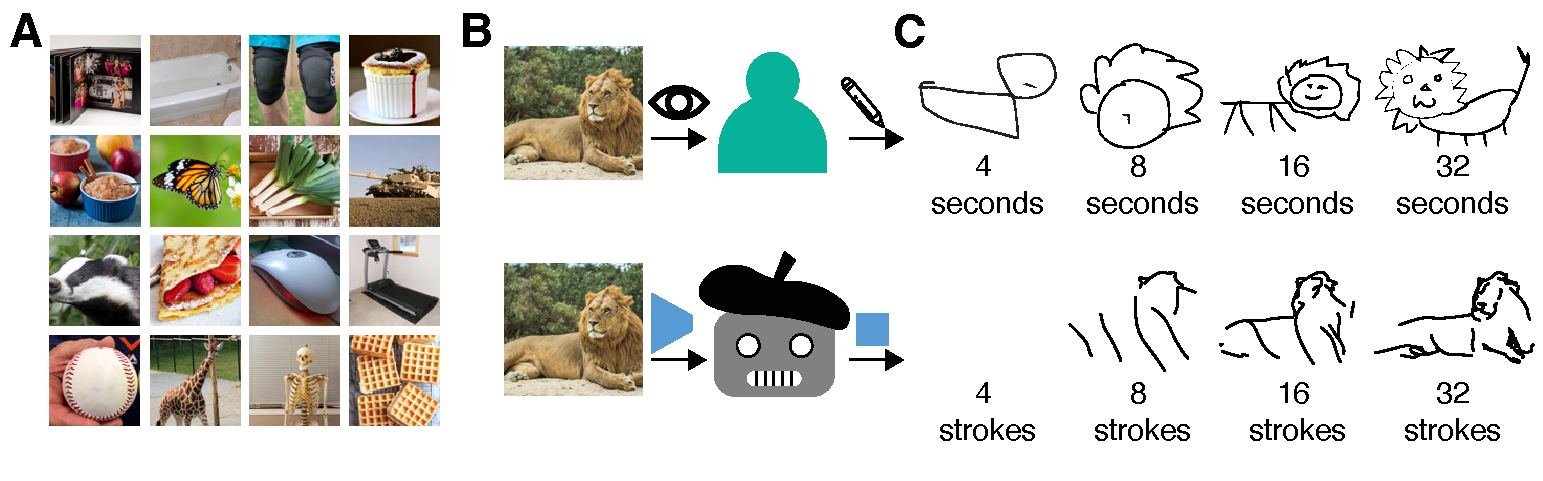
\includegraphics[width= 1\linewidth]{figures/VAB_task.pdf}
 
    \caption{A. Examples of images from the THINGS128 image dataset, a subset of THINGS \cite{hebart2019things}. Each concept had 16 exemplar images that were used as referents in the time-restricted drawing task. B. Both humans and machines were shown the images from THINGS128, but humans were asked to create a sketch of the concept that was represented in photograph while the machine, a CLIP-based generative model \cite{vinker2022clipasso}, used the latent neural features of the image to guide a stroke-based rasterizer. C. Different sources of pressure, limited time in the case of humans and limited number of strokes in the case of the machine, led to sparser drawings in the more pressure-intensive conditions.}

    \label{fig:trial}
\end{figure*}

\subsection{THINGS initiative dataset}
To generate a diverse large-scale stimuli set of object concepts, we systematically sampled 128 concepts from the database of the THINGS initiative, a global database of 1,854 object concepts (e.g., ``chair'', ``elephant'', ``airplane'') and naturalistic object images aimed at developing a multi-varied cognitive neuroscience and behavioral metrics on a shared set of objects \cite{hebart2019things}. 
Building on prior work by \citeauthor{yang2021visual} (2021) investigating visual abstraction across different contexts, we selected concepts based on similar parameters spanning four main axes of variation: familiarity, artificiality, animacy, and size. 
Within each object concept, we randomly sampled 16 object images. 
Our final stimuli set thus included 2,048 object images that were used as visual referents for our human and machine sketching tasks.

\subsection{Human Sketch Production Task} 
\subsubsection{Participants} 
5,563 participants (2,870 male; $M_{age}$ = 36.7 years) were recruited from Prolific to produce a series of sketches on a web-based drawing platform. 
Data collection stopped when 10 sketches had been generated for each of the 2,048 object images.
We excluded 104 data sessions from participants who experienced technical difficulties.
Participants provided informed consent in accordance with our institution’s IRB.

\subsubsection{Procedure}
Participants were randomly assigned to one of four conditions, each varying in the amount of time that they were permitted to use to generate their drawings: 4, 8, 16, or 32 seconds. 
During each drawing trial, participants were presented with a label cue of an object concept, a corresponding object image (500 x 500px) as an example of the concept, and a drawing canvas (500 x 500px) and were instructed to draw the concept that they were presented with (Fig. \ref{fig:trial}). 
Alongside the canvas, participants were given a countdown timer indicating how many seconds they had left to produce their drawing. 
To ensure that participants were prepared to draw given the short duration of each condition, a reminder about the drawing duration was interleaved between drawing trials that also provided participants the opportunity to take a short break and to indicate when they were ready to start the next trial. 
A trial ended when the timer ran out or if the participant pressed the ``Continue'' button if they finished their sketch with time remaining, although they were instructed to try to use as much time as they could to accurately represent the concepts that they were asked to draw.
They were also permitted to undo their most recent stroke or completely clear their canvas if needed. 

Each participant produced 16 drawings of different object concepts.
Prior to drawing trials, participants were provided specific instructions that they were to draw the general concept of presented objects and that, although the provided object image was an example of the concept, they should not include details that were specific to the object in the image. 
Additionally, they were instructed not to include any background context (e.g., grass in a drawing of a ``horse''), arrows, or text.
Participants also completed a practice trial before the test drawing trials to familiarize themselves to the drawing platform.



\subsection{Machine generated sketches}
For the automatic generation of sketches from images at multiple levels of abstraction, we incorporated CLIPasso \cite{vinker2022clipasso}.
CLIPasso is a recently developed method for object sketching, in which the parameters of a predefined set of strokes are optimized to depict a given image of an object, guided by a pre-trained CLIP \cite{radford2021learning} model.
Different levels of abstraction are achieved by varying the number of strokes used. 
For each image in the $2024$ set, we generate sketches at four levels of abstraction using 4, 8, 16, and 32 strokes (see Figure \ref{fig:clipasso_ex} for example).

% We also leveraged recent advances in sketch-generation algorithms, namely the CLIPasso model \cite{vinker2022clipasso}, to generate sketches at different levels of abstraction. 
% We sampled a single exemplar photo for each concept and generated sketches at 3 levels of abstraction for those photos. Since CLIPasso varies abstraction by varying the total number of strokes the model uses to create the sketch we had the model produce sketches with 8, 16, and 32 strokes (Figure \ref{fig:clipasso_ex}. 

% \begin{figure}
%     \centering
%     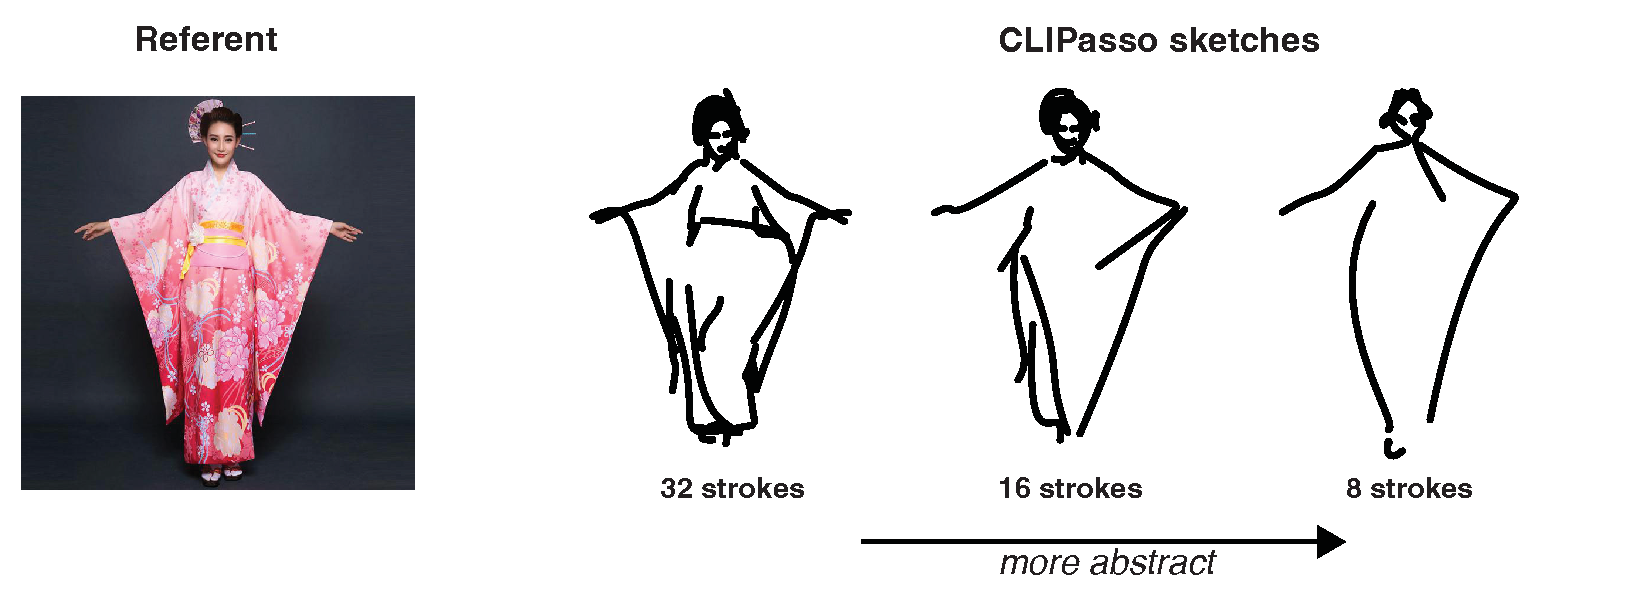
\includegraphics[width=.5\textwidth]{figures/clipasso.pdf}
%     \caption{Machine generated sketches of a photograph at low (32 strokes), medium (16 strokes), and high (8 strokes) levels of abstraction}
%     \label{fig:clipasso_ex}
% \end{figure}

\subsubsection{Results}
We collected over 84,000 unique drawings of the THINGS128 dataset. We first tested whether there were any meaningful differences between the sketches of the same concept across the different timing conditions.
The amount of detailed included in each drawing, measured using the number of unique strokes in a drawing, did increase with increased allowed drawing time with the 4s condition having the fewest strokes and the 32s condition having the most strokes on average. Refer to table \ref{tab:strokes} for information on all 4 conditions.
A mixed-effects linear regression model with random intercepts for concept type predicting number of strokes as a function of time allotted per drawing showed a significant effect of time ($\beta=.029$, $t=58.54$, $p<.001$). Thus, our time-restriction manipulation did indeed lead to drawings that varied in level of detail. In order to answer our questions about visual abstraction, we define two complementary metrics to measure the amount of abstraction in a sketch based on its latent representations. 

\begin{table}[h!]
    \centering
    \begin{tabular}{c|l l}
        Drawing time & $M_{strokes}$ & $SD_{strokes}$\\
         \toprule
        4 seconds & 1.61 & 1.49\\
        8 seconds & 3.49 & 2.43\\
        16 seconds & 6.39 & 4.27\\
        32 seconds & 9.90 & 7.11\\
        \bottomrule 
    \end{tabular}
    \caption{Differences in number of strokes used per drawing condition. Longer drawing times resulted in more detailed drawings, but also a greater variance in amount of detail included }
    \label{tab:strokes}
\end{table}


\section{Formalizing abstraction in vision models}
\begin{figure*}
    \centering
    \includegraphics[width= .95\linewidth]{figures/VAB_models.pdf}
 
    \caption{The general procedure for computing visual abstraction metrics. A. For a given sketch, latent neural network features are extracted for both the sketch and all 2048 images in the THINGS128 image dataset. B.(bottom)  The set of all neural network models benchmarked; we sought to cover models that varied in their training objectives and their architectural backbone. The pairwise cosine feature distances between the input sketch and every image is computed and then normalized to yield empirical distributions of associations at the concept and exemplar level, $P_{concept}$ and $P_{exemplar}$. For each empirical distribution there exists a corresponding 'ideal' target distribution that perfectly represents either the concept, $\delta_{concept}$, or exemplar or $\delta_{exemplar}$ depicted in the sketch. (C) Information from these distributions are leverage to compute our two visual abstraction metrics — specificity and genericity.}

    \label{fig:trial}
\end{figure*}

Beyond object recognition and scene segmentation, robust vision algorithms should be more sensitive to an image's abstractness relative to less human-like algorithms. Further, what properties of a vision model might hinder or facilitate visual abstraction comprehension? In order to answer this question, we curated a set of vision models with a varied architectural commitments and training procedures. We then describe methods for relating latent representations extracted from early, intermediate, and late layers of the models, of sketches to those of the THINGS128 dataset in order to define a formal set of metrics for visual abstraction.

% ... We would like to investigate 1) how models differ in their sensitivities to the level of abstraction and 2) how this ability varies in the early, intermediate, and late representations of vision models. To investigate the   se problems, we first proposed two metrics, specificity and genericity, that quantitatively measure the model sensitivity to variation in abstraction. We then evaluated a variety of vision models with their early/intermediate/late representations and [other analysis].


\textbf{Models}

We evaluated 13 models spanning multiple architectures (ConvNets, Transformers, and MLP), training paradigms (supervised learning, self-supervised learning, and semi-supervised learning), and datasets to disentangle their effects. The models include 3 ImageNet-supervised ConvNets, 3 ImageNet-supervised transformers, 4 self-supervised vision models, CLIP, and two semi-supervised models. Table \ref{tab:models} shows a complete list of the models we benchmarked.

\begin{table}[htp]
\centering
% \vspace{-4mm}
\resizebox{0.5\textwidth}{!}{%
\begin{tabular}{l|l|l|l}
Methods  & Architecture & Training Paradigm & Dataset\\ 
\hline
VGG-19~\cite{} & VGG-19 & supervised & ImageNet\\ 
Inception-V3~\cite{} & Inception-V3 & supervised & ImageNet\\
ResNet-50~\cite{} &  ResNet-50  & supervised & ImageNet \\
ViT-B~\cite{}  & ViT-B & supervised & ImageNet \\
Swin-B\cite{} & Swin-B & supervised & ImageNet \\ 
MLPMixer-B~\cite{} & MLPMixer-B & supervised & ImageNet \\ 
MoCo-v2~\cite{} & ResNet-50 & self-supervised & ImageNet \\ 
MoCo-v3~\cite{} & ViT-B & self-supervised & ImageNet \\ 
DINO~\cite{} & ViT-B & self-supervised & ImageNet \\ 
MAE~\cite{} & ViT-B & self-supervised & ImageNet \\ 
CLIP~\cite{} & ViT-B & self-supervised & WebImageText \\ 
Noisy Student~\cite{} & EfficientNet-b4 & semi-supervised & ImageNet + JFT \\
SWSL~\cite{} &  ResNet-50  & semi-supervised & ImageNet + 1B-Targeted \\
\bottomrule 
\end{tabular}%
}
%\vspace{1mm}
\caption{The list of models that we evaluated. We show the network architecture, training paradigm, and training dataset of each model.}
% \vspace{-5mm}
\label{tab:models}
\end{table}

% Among convolutional models trained using supervised learning we evaluated VGG-19, Inception-V3, and ResNet-50.\\
% Among models trained using self-supervised learning we evaluated SimCLR, BYOL, MoCo, and DINO.\\
% We also evaluated the Vision Transformer (ViT), a transformer-based model trained using supervised learning, and CLIP-ViT, a text-image multimodal model trained using contrastive language-image pretraining.

% \textbf{Genericity and Specificity Metrics} We outline 2 main desiderata for a measure of a sketch's abstractness and ground them in concrete metrics. 
% \begin{itemize}
%     \item \textbf{Genericity} Firstly, if a sketch is abstract, the measure should provide strong evidence for the correct concept (relative to other concepts) but not any specific exemplar of that concept.
%     \item \textbf{Specificity} Secondly, for an abstract sketch, the measure should not provide strong evidence for \textit{any} specific exemplar of \textit{any} concept either.\\
% \end{itemize}

We manually defined and separated each vision model into three stages: early, intermediate, and late. These stages are roughly equivalent to the first 25\% of the layers, the middle 50\% of the layers, and the final 25\% of the layers. 
% See Appendix (?) for the exact split of stages in each model. 
Given an image, we then extracted its latent features at the end of each of these stages as the early, intermediate, and late representation.

\subsubsection{Metrics of visual abstraction} 

We considered two main desiderata for a measure of a sketch's level of abstraction and grounded them in concrete metrics. 
\begin{itemize}

    % \item \textbf{Specificity} Secondly, for an abstract sketch, the measure should not provide strong evidence for \textit{any} specific exemplar of \textit{any} concept either.\\
    \item \textbf{Specificity.} An abstract sketch should not be particularly evocative of any particular exemplar. Here, am sketch should not be highly similar to the referent photo that was displayed during the drawing task.
    Thus, the greater the degree of abstraction in a sketch, the lesser its specificity.    
    \item \textbf{Genericity} If a sketch is abstract, the measure should provide \textit{stronger} evidence for the correct concept depicted in a drawing relative to evidence for a particular instance of that concept. Here, for consistency with specificity, we will operationalize the metric such that more abstraction corresponds to lower genericity score.
    % \item \textbf{Genericity} Firstly, if a sketch is abstract, the measure should provide strong evidence for the correct concept (relative to other concepts) but not any specific exemplar of that concept.

\end{itemize}

In order to mathematically ground our two constructs, we denote $S, E, C$ as the set of sketches, photo exemplars, and concepts, respectively. Given a vision model and a selected early/intermediate/late layer, we extracted the feature embeddings of the $2048$ photo exemplars, denoted $F_{E} \in \mathbb{R}^{2048\times channel}$. Similarly, we extracted the embedding of sketches from the human sketch production set as $F_{S} \in \mathbb{R}^{89419\times channel}$.
% We computed the embedding of each of the 128 concepts as the mean embedding of the 16 photo exemplars corresponding to it, denoted $F_{concept} \in \mathbb{R}^{128 \times c}$.

We use cosine similarity to calculate the similarity between any given sketch $s\in S$ and the 2048 photo exemplars $E$. The resulting similarity matrix $\mathbb{R}^{1 \times 2048}$ is normalized with the softmax function, which gives a probability distribution $P_{E}^{(s)}$ that represents the probability that the sketch corresponds to each of the 2048 photo exemplars. 
% Similarly, we computed the probability distribution $P_{concept}^{(i)}$ that consists of the probability that the sketch corresponds to each concept. 
The similarity matrix between sketch $s$ and the 128 concepts $C$ is computed as the mean similarity between sketch and the 16 photo exemplars corresponding to each concept, giving us the probability distribution $P_{C}^{(s)}$ after softmax.
Formally, we have
\begin{equation}\label{eq:p exemplar}
    P_{E}^{(s)} = \sigma (Similarity(F_{S}^{(s)}, F_{E})),
\end{equation}
\begin{equation}\label{eq:p concept}
    P_{C}^{(s)} = \sigma (\frac{1}{16} \sum_{c\in C}Similarity(F_{S}^{(s)}, F_{E_{\in c}})),
\end{equation}
where $\sigma$ is the softmax function and $Similarity$ is the cosine similarity.

% With the probability distributions ready,
We now detail the formulation of the two metrics.

% To ground these desiderata we first extract deep neural network embeddings for the sketch, which we will refer to as $\textit{s}$, and for each of the 2048 reference images used for the drawing task, which we will refer to as $\textit{I}$.
% Next, we compute the cosine similarities between $s$ and every photo in $I$ and normalize the resulting list of similarity values using the softmax function. We refer to the resulting probability distribution as $p(s)_{instance}$
% $$p(s)_{instance} = \sigma({S_c(s,{I})})$$
% We also compute the normalized average similarity \textit{per category} as follows and refer to the resulting distribution as $p(s)_{concept}$
% $$p(s)_{concept} = \sigma(\frac{1}{16} \sum^{C}_{ c} {S_c(s,{I}_{\in c})})$$

% Both $p(s)_{instance}$ and $p(s)_{concept}$ are probability distributions that indicate how much each sketch evokes each exemplar and, on average, each concept in our dataset respectively.
% We can also imagine \textit{idealized} PDFs for both these PDFs, where all the probability mass is on the exemplar that was the referent when the sketch was made or all the mass on the concept that was prompted when the sketch was made. We refer to these idealized probability distributions as $\delta_{instance}$ and $\delta_{concept}$ respectively. $\delta_{instance}$ can be viewed as the ideal pattern of similarities that would image if a sketch was a perfectly detailed reproduction of a specific exemplar. $\delta_{concept}$ on the other hand is the ideal pattern of similarities that would result from a sketch that is the ideal prototype of the concept, such that it evokes that concept and that concept alone in an observer.

% In order to compute the genericity of a sketch, we measure to what degree it evokes any specific exemplar within its concept category relative to how well it evokes the correct concept.
% The generericty $G$ of sketch $s$ can be defined as -

% $$G(s) = \frac{H(\sigma(S_c(s,{I}_{\in concept(s)})))}{H(p(s)_{concept},\delta_{concept}(s))}$$

% Here, the numerator is the entropy of the pattern of similarities between the sketch and all the exemplar images belonging to the concept the sketch is of. The denominator is the cross entropy between the empirical and idealized concept level PDFs. The smaller this term, the more abstract the given sketch is.

\textbf{Specificity score.} 
% As mentioned in the two desiderata, a highly abstract sketch should not strongly correspond to its photo exemplar. Therefore, 
The specificity metric $L_{Specificity}$ measures how strongly a sketch matches its corresponding photo exemplar, treating all other exemplars as distractors. We formulated the problem as selecting the correct exemplar out of the 2048 photos. Given the sketch $s$ and its correct exemplar $e_{true}^{(s)}\in E$, the metric is computed as the reciprocal of the cross entropy between the one-hot target distribution $\delta^{(s)}$ and the probability distribution $P_{E}^{(s)}$,

\begin{equation}\label{eq:specificity}
    L_{Specificity}^{(s)} =-\frac{1}{\sum_{e\in E}{\delta^{(s)}(e) \log{[P_{E}^{(s)}(e)}]}},
\end{equation}

where 
\begin{equation}\label{eq:one hot}
    \delta^{(s)}(e) :=
    \begin{cases}
1 &\text{if } e = e_{true}^{(s)}, \\
0 &\text{if } e \neq e_{true}^{(s)}.
\end{cases}
\end{equation}



% To compute the specificity of a sketch, we measure the KL-divergence between the idealized and empirical instance level distributions. The larger this term the less abstract a sketch is.

% $$S(s) = D_{KL}(p(s)_{instance},\delta_{instance}(s))$$
% \textbf{Results}



\textbf{Genericity.} 
The genericity metric $L_{Genericity}$ measures how strongly a sketch corresponds to a concept without evoking any particular exemplar within the concept category.
This can be formalized as a ratio between the likelihood of assigning the drawing to the photo that was the referent during the human production experiment and the likelihood of assigning the drawing to the correct category. The smaller this number is, the less likely one is to correctly assign the drawing to the exemplar relative to correctly assigning it to the concept. This would be a drawing that evokes a concept more generally without evoking a particular exemplar.

Given the sketch $s$, its correct exemplar $e_{true}^{(s)}\in E$ and its correct concept $c_{true}^{(s)} \in C$, the metric is computed as the ratio between the cross-entropy between the one-hot target distribution $\delta_{C}^{(s)}$ and probability distribution $P_{C}^_{(s)}$ and the cross-entropy between the one-hot target distribution $\delta_{E}^{(s)}$ and probability distribution $P_{E}^{(s)}$,

\begin{equation}\label{eq:genericity}
    L_{Genericity}^{(s)} =-\frac{\sum_{e\in E}{\delta_{E}^{(s)}(e) \log{[P_{E}^{(s)}(e)}]}}{\sum_{c\in C}{\delta_{C}^{(s)}(c)  \log{[P_{C}^{(s)}(c)}]}},
\end{equation}

where 
\begin{equation}\label{eq:one hot}
    \delta_{E}^{(s)}(e) :=
    \begin{cases}
1 &\text{if } e = e_{true}^{(s)}, \\
0 &\text{if } e \neq e_{true}^{(s)},
\end{cases}
\end{equation}
and
\begin{equation}\label{eq:one hot}
    \delta_{C}^{(s)}(c) :=
    \begin{cases}
1 &\text{if } c = c_{true}^{(s)}, \\
0 &\text{if } c \neq c_{true}^{(s)}.
\end{cases}
\end{equation}



\begin{figure*}[ht!!]
    \centering
    \includegraphics[width=.95\textwidth]{figures/VAB_all_mod.pdf}
    \caption{Average genericity and specificity scores for sketches made in each timing condition based on latent features extracted from each model in our model suite at early, intermediate, and late stages of processing. }
    \label{fig:all_models}
\end{figure*}


\subsection{Results}

\subsection{something about classification}

\begin{figure}
    \centering
    \includegraphics[width=.5\textwidth]{figures/VAB_consistency.pdf}
    \caption{How consistent?}
    \label{fig:consistency}
\end{figure}

\subsection{something about finer metrics}

The full picture of every model being benchmarked along with specificity and genericity metrics derived at early, intermediate, and late stages of processing can be seen in figure \ref{fig:all_models}. Certain general trends can be observed, such as a greater processing of abstraction across the time-restricted conditions in deeper layers of most models captured by a significant positive interaction between model depth $\times$ timing condition (genericity: $\beta_{model\_depth \times time} = $1.69, $t =$21.74, $p<$.05; specificity:$\beta_{model\_depth \times time} = $3.24, $t =$43.05, $p<$.05 ). This aligns with the notion that deeper stages of processing in deep neural networks represent their input in a more categorical manner abstracted away from the specific image statistics of the input \cite{yamins2014performance,khaligh2014deep,rajalingham2018large}. 

While we established that our time-restriction manipulation resulted in less detailed drawings, often a signature of abstraction, for shorter drawing times are these drawings really more abstract? 
To evaluate the hypothesis that shorter drawing times lead to more abstract representations we first investigated whether drawings made under greater time pressure led to more abstract representations in vision models as measured by our abstraction metrics.

A linear mixed-effects model with random intercepts for the referent image concept showed a significant effect of drawing time, with drawings made with more time showing greater specificity ( $\beta =$ 1.79e-05, $t=$ 28, $p<$.05) and also greater genericity ( $\beta =$ 4.05e-05, $t=$ 65.55, $p<$.05).
Thus, as resources such as time become scarce, the more abstract people's depictions of concepts become.

While convolutional neural networks have garnered sustained interest as some of the best performing models of human vision \cite{yamins2014performance,cadieu2014deep,kriegeskorte2015deep,kietzmann2019recurrence}, there have yet to be systematic investigations into the ability of convnets and other vision algorithms to represent the same concept at multiple levels of abstraction on a large-scale dataset such as ours.
Thus we ask, do models that have inductive biases similar to those of human biological vision have an advantage in discerning abstractness in drawings?
We investigated this by asking how model architecture might influence models' ability to represent increasingly sparse sketches across our different drawing time conditions.
We grouped the model architectures broadly into 3 classes — convolution-based models (convnets), transformer-based models, and models relying primarily on multi-layer perceptrons \cite{tolstikhin2021mlp}— and represented abstraction metrics generated from each class of model using dummy codes with convnets as the reference class. We used these predictors in conjunction with drawing time and their interactions to fit a mixed-effects linear regression model with random intercepts per concept predicting both abstractness metrics.
We found that the effect of time-restriction on abstraction was weaker in mlp and transformer architectures relative to convolutional models (figure \ref{fig:gen_spec} (left column)).
This was supported by a significant effect of model class $\times$ timing condition on both the specificity (
$\beta_{mlp \times time}= $ -5.81e-06, $t =$ -24.23, $p<$.05; $\beta_{transformer \times time}= $ -3.19e-06, $t =$ -24.88, $p<$.05) and genericity metrics (
$\beta_{mlp \times time}= $ -3.50e-05, $t =$ -35.12, $p<$.05; $\beta_{transformer \times time}= $-1.92e-05 , $t =$ -24.88, $p<$.05). While transformers continue to drive much progress in natural language process and vision \cite{chen2021visformer}, our results point to the continued relevance of convnets in modeling aspects of human visual cognition.


Along with variations in architecture, a variety of optimization regimes or training techniques have arisen in recent years that have improved model performance on standard benchmarks such as ImageNet classification \cite{deng2009imagenet}. Do these innovations in training protocols bear on our question of visual abstraction? 
To answer this question, we first grouped techniques into 3 classes — supervised learning methods, unsupervised learning methods, and semi-supervised methods (see table \ref{tab:models} for a full list). Once again we dummy coded these conditions, treating supervised learning as the reference class and fit a linear-mixed effects model in the same manner as we did for architecture, replacing those terms with terms for training techniques. The interaction of training technique $\times$ timing condition for both semi-supervised and unsupervised was positive in both the specificity ($\beta_{supervised \times time}= $ 1.17e-06, $t =$ 8.77, $p<$.05; $\beta_{semi-supervised \times time}= $ 9.03e-06, $t =$ 49.90, $p<$.05) and genericity model $\beta_{supervised \times time}= $ 6.76e-06, $t =$12.13, $p<$.05; $\beta_{semi-supervised \times time}= $ 5.54e-05 , $t =$ 73.70, $p<$.05).
While both metrics point towards semi-supervised and self-supervised training methods better capturing the effect of time-restriction on abstraction, as can be seen in figure \ref{fig:gen_spec} (right column), the magnitude of this effect is greatly pronounced for representations derived from models trained using semi-supervised techniques.



\begin{figure}
    \centering
    \includegraphics[width=.5\textwidth]{figures/VAB_gen_spec.pdf}
    \caption{The effect of architecture (left) and training algorithm (right) on visual abstraction metrics. }
    \label{fig:gen_spec}
\end{figure}


\section{Discussion}

\section{Acknowledgments}

% The authors would like to thank members of the Cognitive Tools Lab at UC San Diego for their comments and support. This work was supported by NSF CAREER Award #2047191 to J.E.F.


\bibliographystyle{apacite}

\setlength{\bibleftmargin}{.125in}
\setlength{\bibindent}{-\bibleftmargin}

\bibliography{references}


\end{document}
